\documentclass[12pt,a4]{article}



\newcommand{\handoutdate}{Monday, 2019-10-21}
\newcommand{\firstduedate}{Monday, 2019-10-28}
\newcommand{\finalduedate}{Monday, 2019-11-04}




\usepackage{graphicx,amsmath,amssymb,amsthm, boxedminipage}



\usepackage{algorithm}
\usepackage{algpseudocode}


\newtheorem{theorem}{Theorem}%[section]
\newtheorem{proposition}[theorem]{Proposition}
\newtheorem{lemma}[theorem]{Lemma}
\newtheorem{corollary}[theorem]{Corollary}
\newtheorem{definition}[theorem]{Definition}



\newcommand{\scalar}[2]{\ensuremath{\langle #1, #2\rangle}}
\newcommand{\floor}[1]{\left\lfloor #1 \right\rfloor}
\newcommand{\ceil}[1]{\left\lceil #1 \right\rceil}
\newcommand{\norm}[1]{\|#1\|}
\newcommand{\pfrac}[2]{\left(\frac{#1}{#2}\right)}
\newcommand{\nth}[1]{#1\textsuperscript{th}}

% \newcommand{\nth}[1]{#1\textsuperscript{th}}
\newcommand{\E}{\mathop{\mathbb{E\/}}}
\newcommand{\N}{\mathbb{N}}

\newcommand{\R}{\mathbb{R}}

\newtheorem{exercise}[theorem]{Exercise}
\newtheorem{exerciseD}[theorem]{*Exercise}
\newtheorem{exerciseDD}[theorem]{**Exercise}

\let\oldexercise\exercise
\renewcommand{\exercise}{\oldexercise\normalfont}

\let\oldexerciseD\exerciseD
\renewcommand{\exerciseD}{\oldexerciseD\normalfont}

\let\oldexerciseDD\exerciseDD
\renewcommand{\exerciseDD}{\oldexerciseDD\normalfont}


 
\begin{document}

\date{}

\title{CS 217 -- Algorithm Design and Analysis \\ 
  \vspace{3mm}
{\large	Shanghai Jiaotong University, Fall 2019\\
}
}
\maketitle

\noindent
Handed out on \handoutdate{}\\
First submission and questions due on \firstduedate{}\\
You will receive feedback from the TA.\\
Final submission due on \finalduedate{}




\setcounter{section}{4}
\section{More on Network Flows}

\begin{exercise}
    Let $G = (V,c)$ be a flow network. Prove that flow is ``transitive'' in the following sense: if $r,s,t$ are vertices, 
    and there is an $r$--$s$-flow of value $k$ and an $s$--$t$-flow of value $k$, then there is an $r$--$t$-flow of 
    value $k$.
\end{exercise}

\begin{proof}
	Denote the original r-s-flow and s-t-flow as $f_{rs}$ and $f_{st}$ respectively.
    We prove $f_{rt} = k$ by contradiction.

    Suppose $f_{rt} < k$, denote $f_{rt} = p$. By Max-Flow-Min-Cut THM, there is a cut $C$ 
    with $cap(C) = p < k$. If $s \in C$, we know that $C$ is also a r-s-cut. But by Max-Flow-Min-Cut
    THM, min $cap(r-s-cut) = k > cap(C) = p$, which leads to a contradiction. If $s \notin C$, the proof
    is similar. So $f_{rt} \ge k$, so there is a flow of value k in between $r, t$.
	
\end{proof}

\subsection{Vertex Disjoint Paths}

Let $G$ be a directed graph. Two paths $p_1, p_2$ from $s$ to $t$ are called {\em vertex disjoint}
if they don't share any vertices except $s$ and $t$. 

\begin{theorem}[Menger's Theorem]
   Let $G$ be a graph and $s \ne t$ two vertices therein. Let $k \in \mathbf{N}_0$. 
   Then exactly one of the following is true:
   \begin{enumerate}
   \item There are $k$ vertex disjoint paths $p_1,\dots,p_k$ from $s$ to $t$; that is, no two $p_i$, $p_j$ share
   any vertex besides $s$ and $t$.
   \item There are vertices $v_1,\dots,v_{k-1} \in V \setminus \{s,t\}$ such that
   $G - \{v_1,\dots, v_{k-1}\}$ contains no $s$--$t$-path.
   \end{enumerate}
\end{theorem}

\begin{exercise}
   Prove Menger's Theorem. You have to prove two things: first, not both cases above can occur (this is rather easy);
   second, one of them must occur (this requires a tool from the lecture).
\end{exercise}
\begin{proof}
    First we prove the easy part, these two cases will not occur simultaneously.Prove it by contradiction.

    Suppose both cases are true simultaneously, then there are $k$ vertex disjoint paths $p_1, ..., p_k$ from $s$ to $t$.
    and there exists $v_1, ..., v_{k - 1}$ such that $G - \{ v_1, ...,v_{k - 1}\}$ contains no 
    s-t-path. 
    
    For any $v_1, ..., v_{k - 1}$, the can take place in at most $k - 1$ paths in $p_1,...,p_k$ since $p_1, ..., p_k$ are
    disjoint vertex paths. Then we know there must be at least one path from $p_1,..,p_k$ left, which connects $s$ and $t$,
    leading to a contradiction.


    Next we prove that one of them must occur.

    The second case is obvious since we can just remove all vertices except $s, t$ from the $V$, then obviously there're no
    s-t-path now.

    For the first case, we construct such a network-graph with all edge in the original graph assigned capacity 1.
    \begin{figure}[h]
        \centering
        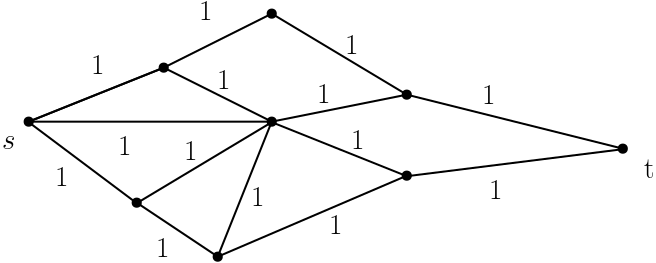
\includegraphics[scale=0.3]{figures/123.png}
        \caption{network}
    \end{figure}
    In such a network, the value of a flow is the number of vertex disjoint paths in such a flow. 
    Since the capacity of each edge is $1$, we can know for sure that no two s-t-path cross with each other,
    otherwise there must be a vertex with units bigger than 1. Based on that, we see $k$, the value of a flow 
    is the number of paths in it. Thus leading to $k$ disjoint paths.

    In fact, we can prove that the maximum number of disjoint paths  is equal to the minimum number of vertex set which
    separates $s, t$.

    We construct a new network from original graph. For a vertex $v$ other than $s, t$, we split it to $v^+, v^-$, and draw a 
    new directed edge $v^-v^+$. For an edge $(s, v)$, replace it with $sv^-$. For an edge $(v, t)$, 
    replace it with $v^+t$. For other edges $(u, v)$, replace it with $(u^+v^-, v^+u^-)$. All new edges are assigned capacity 1.
    Here's an example.

    \begin{figure}[h]
        \centering
        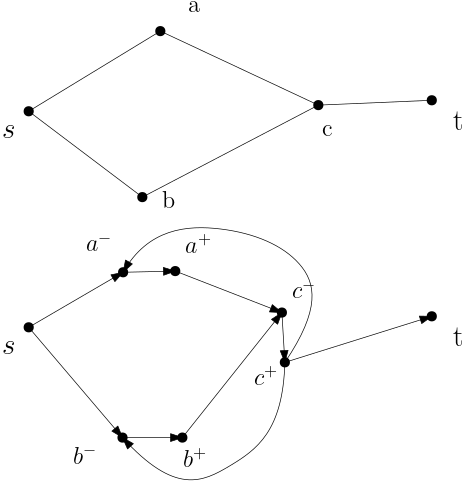
\includegraphics[scale=0.3]{figures/12.png}
        \caption{network}
    \end{figure}

    In such a network $G'$, we split the nodes and put directed edge to make sure no two flow cross each other at some nodes.
    Also, any flow $f$ in this network can produce a set $P$ of disjoint $(s, t)$ paths, $|P| = val(f)$. 
    We add an edge $(u, v)$ to a path if $(u^+, v^-)$ is in the flow.
    Any cut $C$ has a sub set $C'$ with all arcs like $(v^-,v^+)$, and $C'$ still a cut in $G'$. Then we can produce 
    a set of vertices $V$ in $G$ with all nodes $v$($(v^-, v^+) \in C'$).

    Then we know that for a maximum set $P'$of disjoint paths in $G$, $|P'| \ge |P| = val(f) = |C| \ge |C'| \ge |V| \ge |P'|$
    So all of these values are equal, which finishes the proof.

\end{proof}


Let $V = \{0,1\}^n$. The $n$-dimensional Hamming cube $H_n$ is the graph $(V,E)$ where
$\{u,v\} \in E$ if $u,v$ differ in exactly one coordinate.
Define the $\nth{i}$ level of $H_n$ as 
\begin{align*}
  L_i := \{u \in V \ | \ \norm{u}_1 = i \} \ ,
\end{align*}
i.e., those vertices $u$ having exactly $i$ coordinates which are $1$.
\begin{center}
  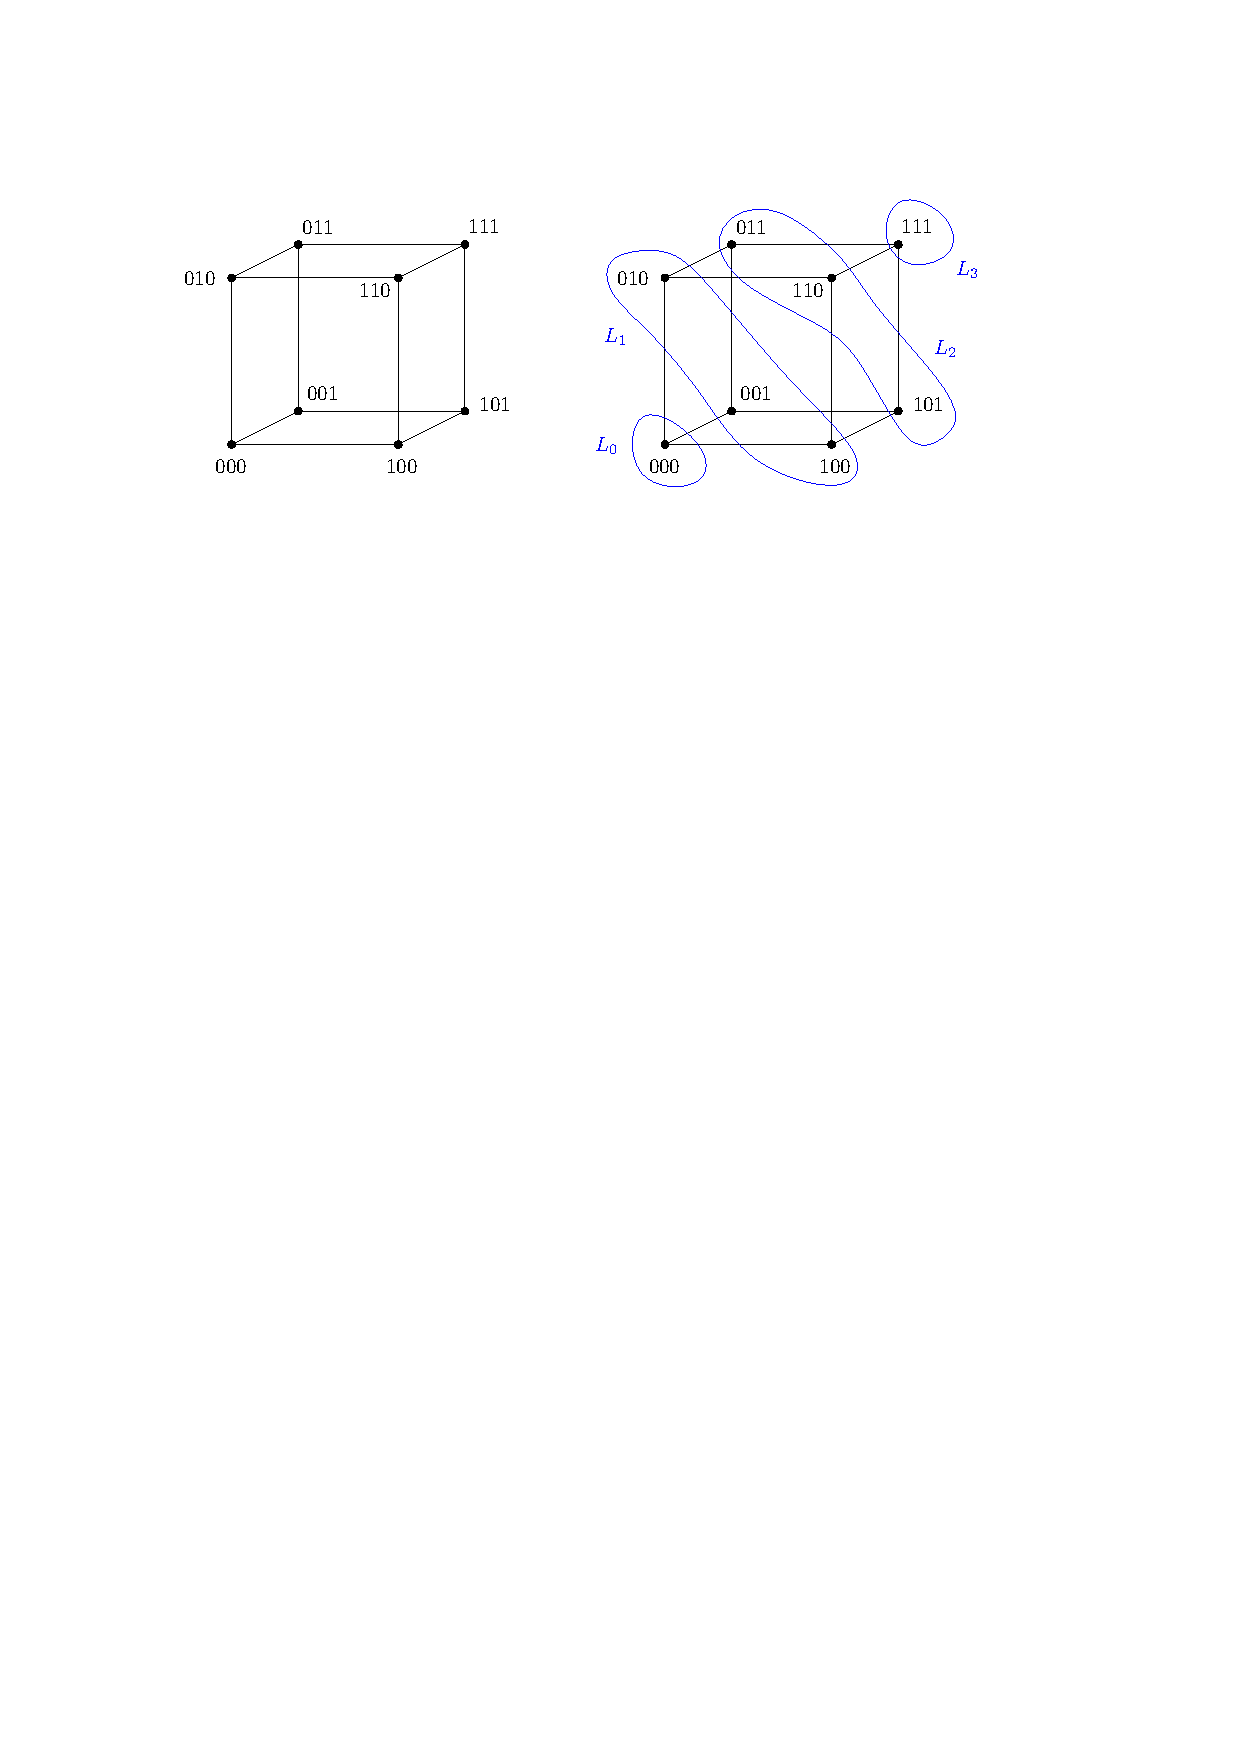
\includegraphics[width=0.8\textwidth]{figures/hamming-3-dim.pdf}\\
  {\small The $3$-dimensional Hamming cube and the four 
    sets $L_0$, $L_1$, $L_2$, $L_3$.}
\end{center}


\begin{exercise}[Matchings in $H_n$]
  Consider the induced bipartite subgraph $H_n[ L_i \cup L_{i+1}]$. This is 
  the graph on vertex set $L_i \cup L_{i+1}$ where two edges are connected
  by an edge if and only if they are connected in $H_n$.
  \medskip

  Show that for $i \leq n/2$ the graph $H_n[ L_i \cup L_{i+1}]$
  has a matching of size $|L_i| = {n \choose i}$.

\begin{center}
  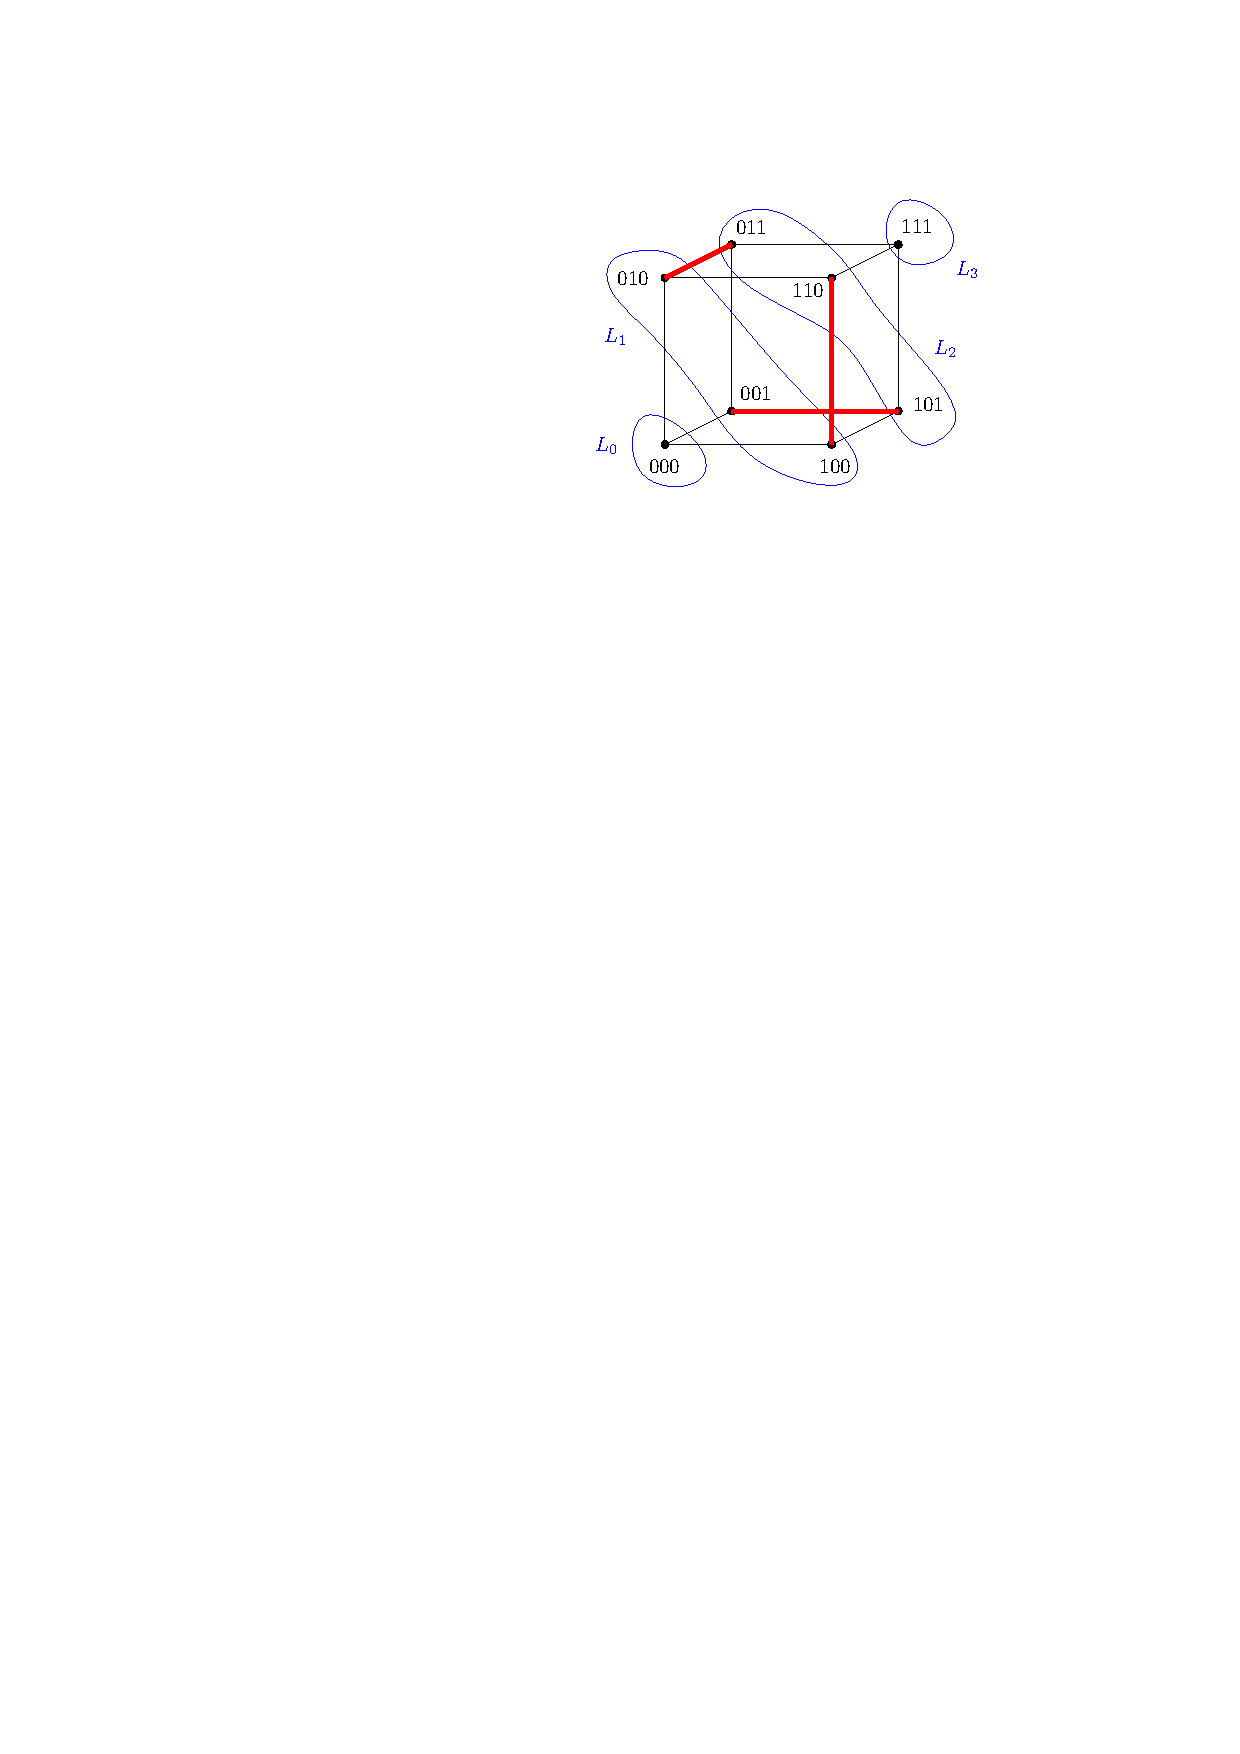
\includegraphics[width=0.4\textwidth]{figures/hamming-3-dim-matching.pdf}\\
  {\small A matching of size $3$ between $L_1$ and $L_2$.}
\end{center}
\label{exercise-matchings-in-H}
\end{exercise}
\begin{proof}
\end{proof}
\begin{exercise} 
  Let $H_n$ be the $n$-dimensional Hamming cube. For $i < n/2$ consider
  $L_i$ and $L_{n-i}$. Note that 
  $|L_i| = {n \choose i} = { n \choose n-i}  = L_{n-i}$, so the 
  $L_i$ and $L_{n-i}$ have the same size.   Show that there are ${n \choose i}$ paths $p_1,p_2,\dots,p_{ {n \choose i}}$
  in $H_n$ such that
  (i) each $p_i$ starts in $L_i$ and ends in $L_{n-i}$;
  (ii) two different paths $p_i,p_j$ do not share any vertices.
  \textbf{Hint 1.} Model this problem as a network flow with vertex capacities. What would 
  the maximum flow be in this network?
  \textbf{Hint 2.} It's not {\em that} easy. If you try to work from both sides towards
  the middle by combining matchings between levels, 
  you will certainly run into problems as how to glue things together in the middle.
  I have never seen any ``meet in the middle'' proof that works.
  \textbf{Hint 3.} There is a ``direct'' proof by induction that does not require anything
  about network flows.

\end{exercise}
\begin{proof}
\end{proof}

\subsection{Matchings and Vertex Covers}

The following exercise was on the final exam of CS 499 (mathematical foundations of computer science) in spring 2019.
\begin{exercise}
    Let $\nu(G)$ denote the size of a maximum matching of $G$. Show that a bipartite graph $G$
    has at most $2^{\nu(G)}$ minimum vertex covers.
\end{exercise}
\begin{proof}

		Suppose the number of minimum vertex covers of graph $G$ is $m\left( G \right) $. We can easily 
\begin{figure}[ht]
    \centering
	\incfig[0.5]{example}
    \caption{example}
    \label{fig:example}
\end{figure}
Now we prove that there could be no more than $2^{\nu \left( G \right) }$ minimum vertex cover.
Let $G = A \cup B$, since $G$ is a bipartite graph. 
Assume that the maximum matching is $e_1,e_2,\ldots,e_t$, in which $t = \nu\left( G \right) $. By \textbf{Konig's Theorem} we know that the number of vertices in a minimum vertex cover is exactly $t$. 

Plus we can prove that every vertex in $K$, the vertex cover, is an endpoint of a matched edge. Hence the result is obvious.
\end{proof}
Obviously, this is not  true for general (non-bipartite) graphs: the triangle $K_3$ has $\nu(K_3) = 1$ but it has 
three minimum vertex covers. The five-cycle $C_5$ has $\nu(C_5) = 2$ but has five minimum vertex covers.

\begin{exercise}
   Is there a function $f: \mathbf{N}_0 \rightarrow \mathbf{N}_0$ such that every graph with $\nu(G) = k$ has 
   at most $f(k)$ minimum vertex covers? How small a function $f$ can you obtain?
\end{exercise}
\begin{proof}
	Since this is for every graph. First consider $K_{2r+1}$, we have $\frac{k}{r}$ $K_{2r+1}$.
	Hence $\nu\left( G \right) = \frac{k}{r} \cdot r = k$
	\[
			f\left( k \right)  \ge  \left( 2r+1 \right) ^{\frac{k}{r}}
	.\] 
	For example, if we choose $r=1$, there are $k$  $K_3$, we have  $f\left( k \right) \ge  3^{k}$. And  let $r\to \infty$  we have 
	\[
			f\left( k \right) \ge  e^{2k}
	.\] 
	Next we prove that the number of minimum vertex cover is at most $e^{2k}$. 
	Consider $\forall $ minimum vertex cover $K$. We prove 
	 \[
	\left| K \right| \le e^{2k}
	.\] 
	Let $\forall u,v \in K$. If $u,v$ are connected, then at least one of them 
	is on a edge of maximum matching.
\end{proof}





\end{document}
